% !TeX root = prob.tex

%%%%%%%%%%%%%%%%%%%%%%%%%%%%%%%%%%%%%%%%%%%%%%%%%%%%%%%%%%%%%%%%

\documentclass[11pt,a4paper]{article}

\usepackage{mathpazo}
\usepackage{microtype}
\usepackage{url}
\usepackage{graphicx}

% TikZ package
\usepackage{tikz}
\usetikzlibrary{arrows.meta}
\tikzset {>=Stealth}


% Displaystyle for fractions and combinations
\newcommand*{\disfrac}[2]{\displaystyle\frac{#1}{#2}}
\newcommand*{\dischoose}[2]{\displaystyle{#1 \choose #2}}

% Change LaTeX defaults for figures
\renewcommand{\topfraction}{0.9}
\renewcommand{\bottomfraction}{0.8}
\setcounter{topnumber}{1}
\setcounter{bottomnumber}{2}
\setcounter{totalnumber}{3}
\renewcommand{\textfraction}{0.07}
\renewcommand{\floatpagefraction}{0.7}

% Layout
\textwidth=150mm
\textheight=225mm
\topmargin=0pt
\headheight=11pt
\oddsidemargin=1em
\evensidemargin=0mm
\headsep=0pt
\parindent=0pt
\renewcommand{\baselinestretch}{1.1}
\setlength{\parskip}{0.3\baselineskip plus 1pt minus 1pt}

%\includeonly{}

\begin{document}

% !TeX root = prob.tex

%%%%%%%%%%%%%%%%%%%%%%%%%%%%%%%%%%%%%%%%%%%%%%%%%%%%%%%%%%%%%%%%

\thispagestyle{empty}

\begin{center}
\textbf{\LARGE Probability Simulations}

\bigskip
\bigskip
\bigskip

\textbf{\Large Moti Ben-Ari}

\bigskip

\url{http://www.weizmann.ac.il/sci-tea/benari/}

\bigskip
\bigskip
\bigskip

%Version $1.1$
%
%\bigskip

\today

\end{center}

\vfill

\begin{center}
\copyright{} Moti Ben-Ari $2023$
 \end{center}
 
\begin{small}
This work is licensed under Attribution-ShareAlike 4.0 International. To view a copy of this license, visit \url{http://creativecommons.org/licenses/by-sa/4.0/}.
\end{small}
\newpage

\tableofcontents

\newpage

\begin{center}
\textbf{\LARGE Introduction}
\end{center}

\addcontentsline{toc}{section}{\large Introduction}

\bigskip

Simulations are an excellent way of understanding probability, especially, the behavior of process of long duration. These programs enable the user to perform experiments by varying the parameters of problems and analyzing the results, both printed and displayed in graphs. A level of knowledge of probability equivalent to the first few chapters of \cite{BW} or \cite{ross} is assumed.

The simulations are of processes known as \emph{Markov chains}, where the next state of the system depends only on the current state and not on the history of how the process got to the current state. These problems appear in probability textbooks \cite{BW, ross} and in much greater detail in \cite{mosteller, mos, border, privault}.

Parameters such as the probability can be modified interactively in order to see how the outcome depends on the values of the parameters.

Section~\ref{s.gamblers} presents the \emph{Gambler's ruin} while Section~\ref{s.walk} presents the one-dimensional \emph{Random walk}.

\subsection*{Technical notes}

The programs are written in the Python 3 language and use the \verb+matplotlib+ to generate the graphs. Parameters directly related to the problems, such as the probability of success, can be modified interactively. Others, related to the simulation, such as the number of steps in a simulation and the properties of the histograms, are defined in a module \verb+configuration.py+ that can be modified.

You need to install the Python (\url{https://www.python.org/downloads/}) although a knowledge of Python programming is not necessary.

To run in the Visual Studio Code environment, ensure that the \verb+Code Runner+ extension is installed. I recommend that in the extension settings disable \verb+Preserve Focus+ and enable \verb+Run In Terminal+.

To run in the IDLE or Thonny environments, change the configuration constant \verb+CLOSE+ to \verb+True+. When the simulation is run multiple times, you will have to close each figure before running a new simulation.

% !TeX root = prob.tex

\section{Gambler's Ruin}\label{s.gamblers}

\textbf{Problem} Two players $A$ and $B$ compete in a contest. There is an initial finite capital of $n$ units: $A$ has $i$ and $B$ has $n-i$. They repeatedly play a game where the probability that $A$ wins is $p$ and the probability that $B$ wins is $q=1-p$. The loser gives one unit to the winner. When one player has all $n$ units the contest is finished.
\begin{enumerate}
\item Given initial parameters $(p, n, i)$, what is the probability that $A$ wins?
\item What is the expected duration of the game?
\end{enumerate}
\begin{center}
\begin{tikzpicture}[scale=1.2]
\draw (0,0) node[above left] {$A$} -- 
      (10,0) node[above right] {$B$};
\foreach \x in {0,1,2,3,4,5,6,7,8,9,10} {
  \draw (\x,0) -- +(0,4pt);
  \node at (\x,-10pt) { $\x$ };
}
\node at (4,-9mm) {$i$};
\node at (10,-9mm) {$n$};
\draw[fill] (4,7mm) circle[radius=1pt];
\draw[->] (4,7mm) -- node[above] {$q$} +(-1,0);
\draw[->] (4,7mm) -- node[above] {$p$} +(1,0);
\end{tikzpicture}
\end{center}
The most extensive presentation the gambler's ruin is in 
\cite[Chapter~2]{privault} which includes the solution to the expected duration of the contest. Note that Privault asks for the probability that $A$ is ruined, that is, that $B$ wins. I follow other references which ask for $A$'s probability of winning.

\subsection{Theoretical results}

Given $(p,n,i)$ the probability that $A$ wins the contest is:
\[
P_A(p, n, i) = \left(\frac{1-r^{i}}{1-r^n}\right)\,,
\]
where $r=q/p$. By symmetry, the probability that $B$ wins is:
\[
P_B(p, n, i) = \left(\frac{1-(1/r)^{n-i}}{1-(1/r)^{n}}\right)\,.
\]

There are separate solutions for $p\neq 1/2$ and $p=1/2$. For $p\neq 1/2$ the expected duration of the contest is:
\[
E_{\mathit{duration}}(p,n,i)=\frac{1}{q-p}\left(i-n
\frac{1-r^k}{1-r^n}\right)\,.
\]
For $p=1/2$ the expected duration of the contest is:
\[
E_{\mathit{duration}}(p,n,i)=i(n-1)\,.
\]
Of course the duration does not depend on which player wins. If $A$ wins, the contest terminates for $B$ also, and conversely.

\subsection{Program structure}

\verb+configuration.py+ contains declarations of variables which are intended to be constant.

\verb+gambler_plot.py+ contains the functions for plotting the histogram of the duration of the contests. If the simulation is run for multiple probabilities or initial values, a graph of the proportion of wins is also displayed.

\verb+gamblers_ruin.py+ is the main program which obtains the parameters, runs the simulations, prints the output and calls the plotting functions.

\subsection{Running the simulations}

The program runs the simulations in a loop, each time asking the user how to run it. You can run the same simulation again with the saved parameters, enter new parameters, or run a sequence of simulations for a range of probabilities or initial values.

A typical output is as follows:
\begin{verbatim}
Probability = 0.45, capital = 20, initial = 8
Wins = 789, losses = 9211, limits exceeded = 0
Proportion of wins     = 0.0789
Probability of winning = 0.0732
Average duration  = 65
Expected duration = 65
\end{verbatim}
The results of the simulation are very close to the theoretical probability and expected duration. The proportion of wins and the histogram of the durations are shown in Figures~\ref{f.gambler-hist1}, \ref{f.gambler-hist2}. The vertical lines are the average durations.

\begin{figure}
\begin{center}
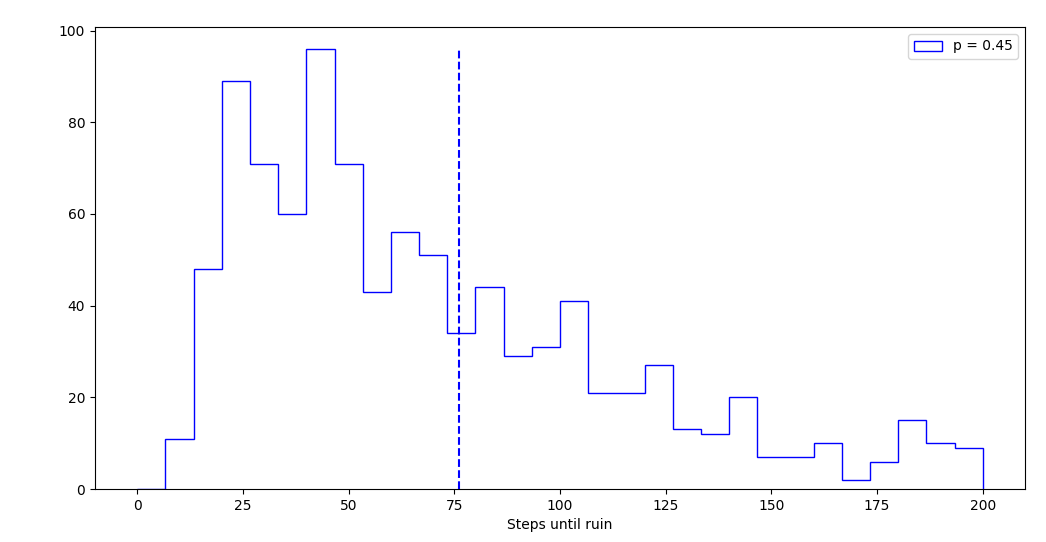
\includegraphics[width=\textwidth]{gamblers_ruin-01}
\caption{Proportion of wins and histogram for $n=20, i=10$ and multiple probabilities}\label{f.gambler-hist1}
\end{center}
\end{figure}

\begin{figure}
\begin{center}
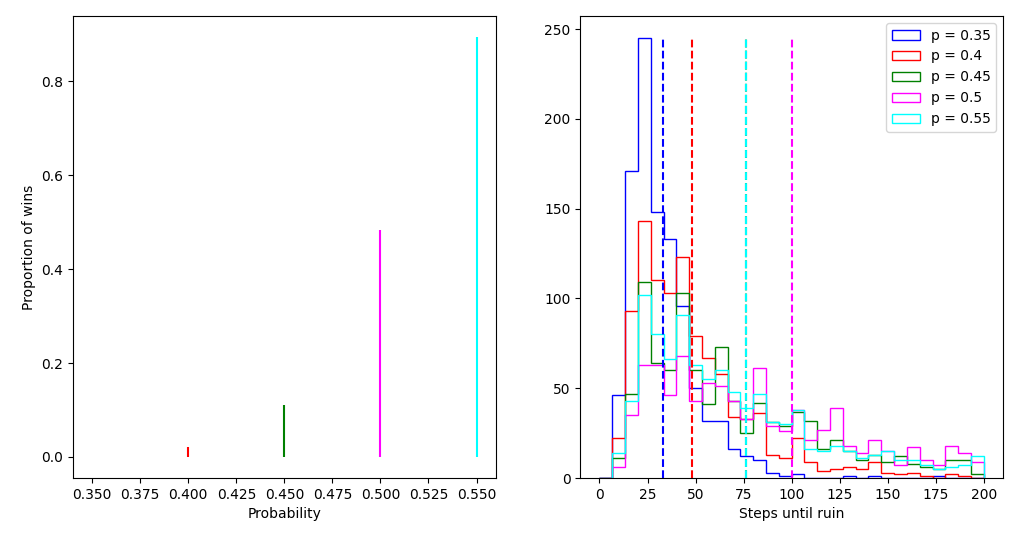
\includegraphics[width=\textwidth]{gamblers_ruin-02}
\caption{Proportion of wins and histogram for $p=0.45, n=20$ and multiple initial values}\label{f.gambler-hist2}
\end{center}
\end{figure}

% !TeX root = prob.tex

\section{Random Walk}\label{s.walk}

\textbf{Problem} A particle is placed at the origin of the $x$-axis. It repeatedly takes steps: right with probability $p$ and left with probability $q=1-p$.
\begin{enumerate}
\item What is the probability that the particle will return to the origin?
\item What is the expected duration until the particle returns to the origin?
\end{enumerate}
\begin{center}
\begin{tikzpicture}[scale=1.2]
\draw[<->] (-6,0) -- (6,0);
\foreach \x in {-5,-4,-3,-2,-1,0,1,2,3,4,5} {
  \draw (\x,0) -- +(0,4pt);
  \node at (\x,-10pt) { $\x$ };
}
\draw[fill] (0,7mm) circle[radius=1pt];
\draw[->] (0,7mm) -- node[above] {$q$} +(-1,0);
\draw[->] (0,7mm) -- node[above] {$p$} +(1,0);
\end{tikzpicture}
\end{center}
The clearest presentation of one-dimensional random walk is in \cite{border}, but the derivation of the expected duration is in \cite{privault}.

\subsection{Theoretical results}

By symmetry, without loss of generality let the first step be to the right. 

The particle can only return to the origin after an even number of steps. Assume that $p=1/2$. Let $S_{2m}$ be the position of the particle after $2m$ steps. Then:
\[
P(S_{2m}=0) = \dischoose{2m}{m}\disfrac{1}{2^{2m}}\,,
\]
which by Stirling's formula is:
\[
P(S_{2m}=0) \approx \disfrac{1}{\sqrt{\pi m}}\,.
\]
It can now be proved that the probability of a return to the origin is $1$.

For $p\leq 1/2$, $P_{\mathit{origin}}$, the probability of a return to the origin, is $1$ and for $p\geq 1/2$ the probability is (Figure~\ref{f.walk1}):
\[
P_{\mathit{origin}} = \disfrac{q}{p}=\disfrac{1-p}{p}\,.
\]
\begin{figure}
\begin{center}
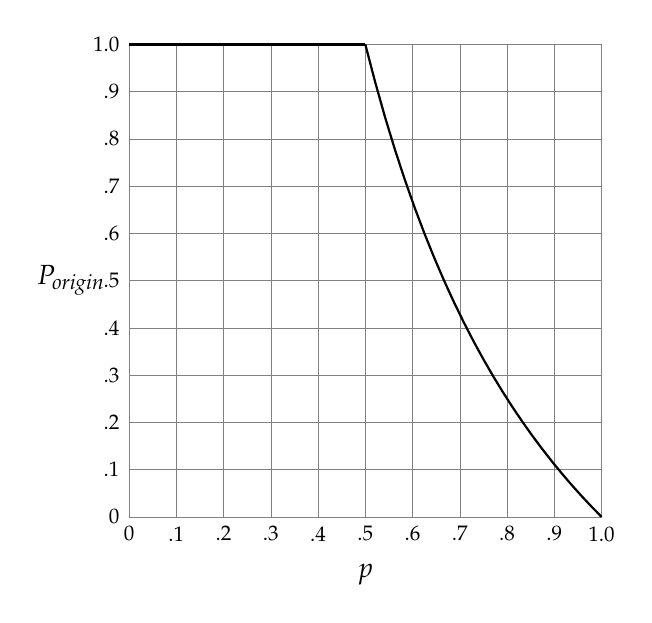
\begin{tikzpicture}[scale=6]
\draw[help lines,step=.1] (0,0) grid (1,1);
\foreach \x in {0,.1,.2,.3,.4,.5,.6,.7,.8,.9,1.0}
  \node[below] at (\x,0) {$\scriptstyle \x$};
\foreach \y in {0,.1,.2,.3,.4,.5,.6,.7,.8,.9,1.0}
  \node[left] at (0,\y) {$\scriptstyle \y$};
\draw[domain=0:.5,thick] plot (\x,1);
\draw[domain=.5:1,thick] plot (\x,{(1-\x)/\x});
\node at (.5,-3.5pt) {$p$};
\node at (-3.5pt,.5) {$P_{\mathit{origin}}$};
\end{tikzpicture}
\caption{Graph of $P_{\mathit{origin}}$}\label{f.walk1}
\end{center}
\end{figure}

$E_{\mathit{origin}}$, the expected duration until the first return to the origin, is infinite for $p\geq 1/2$ while for $p<1/2$ it is:
\[
E_{\mathit{origin}}=\disfrac{1}{q-p}=\disfrac{1}{1-2p}\,.
\]

\subsection{Program structure}

\verb+configuration.py+ contains declarations of variables which are intended to be constant.

\verb+random_walk_plot.py+ contains the functions for plotting a graph of the proportion of simulations that return to the origin and the mean duration if the simulation is run for multiple probabilities or limits.

\verb+random_walk.py+ is the main program which obtains the parameters, runs the simulations, prints the output and calls the plotting functions.

\subsection{Running the simulations}

The program runs the simulations in a loop, each time asking the user how to run it. You can run the same simulation again with the saved parameters, enter new parameters, or run a sequence of simulations for a range of probabilities or limits.

A typical output is as follows:
\begin{verbatim}
Probability = 0.50, step limit   = 1000
Proportion returning to origin   = 0.977
Probability of return to origin  = 1.000
Proportion reaching limit        = 0.023
Mean duration (steps)            = 49
Expected duration (steps)        = infinity
\end{verbatim}
The proportion of wins in the simulation are very close to the theoretical probability, but the mean duration is far from infinite because the step limit was too small.  The proportion of wins and the mean durations are shown in Figures~\ref{f.random_walk-01} and \ref{f.random_walk-02}.
\begin{figure}
\begin{center}
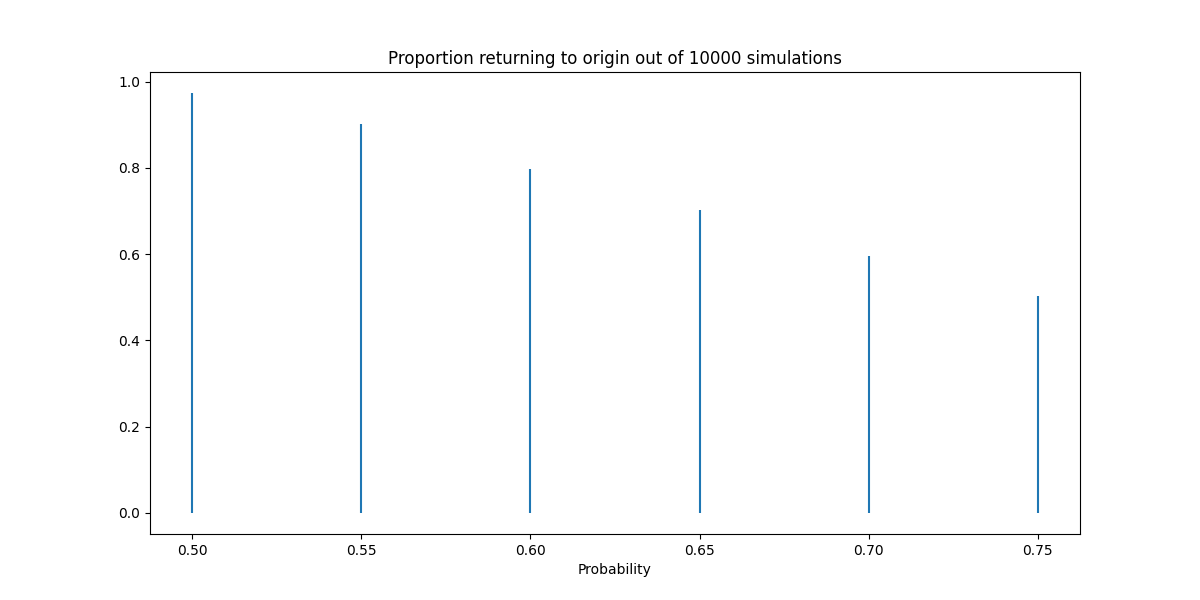
\includegraphics[width=\textwidth]{random_walk-01}
\caption{Proportion of wins and and mean durations for multiple probabilities}\label{f.random_walk-01}
\end{center}
\end{figure}
\begin{figure}
\begin{center}
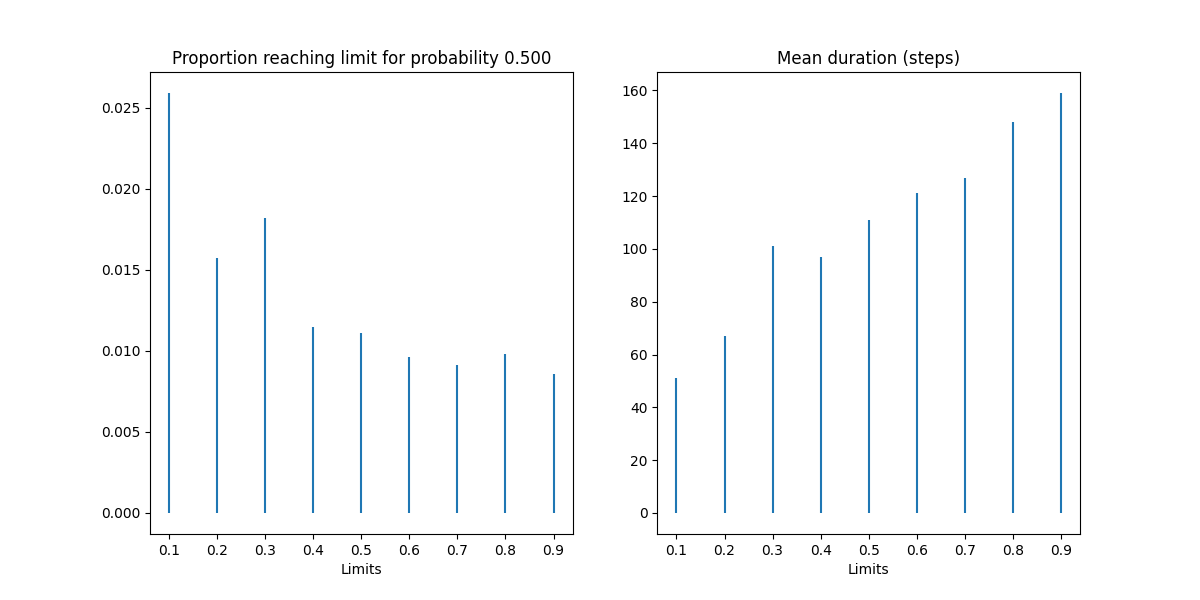
\includegraphics[width=\textwidth]{random_walk-02}
\caption{Proportion of wins and and mean durations for multiple limits}\label{f.random_walk-02}
\end{center}
\end{figure}

% !TeX root = mos-en.tex

\addcontentsline{toc}{section}{\large References}

\bibliographystyle{plain}
\bibliography{prob}


\end{document}
